\documentclass[12pt]{article}
\usepackage{tikz}
\usepackage{circuitikz}
\usepackage{amsmath}
\usepackage{amssymb}
\usepackage{graphicx}
\usepackage{float}
\usepackage{geometry}
\usepackage{pgfplots}
\usepackage{color}
\usepackage{xcolor}

\geometry{a4paper, margin=1in}
\pgfplotsset{compat=1.18}

\begin{document}

Consider the equilibrium:

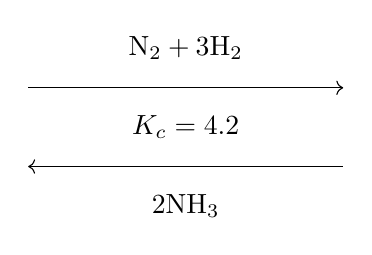
\begin{tikzpicture}
\draw[->] (0,1) -- (4,1);
\draw[<-] (0,0) -- (4,0);
\node at (2,1.5) {$\text{N}_2 + 3\text{H}_2$};
\node at (2,-0.5) {$2\text{NH}_3$};
\node at (2,0.5) {$K_c = 4.2$};
\end{tikzpicture}

If [N₂] = 0.5M and [H₂] = 0.3M at equilibrium:
Calculate [NH₃] at equilibrium.

\end{document}
